\section{Surface Parameterization Methods}


This package provides a second \ccc{parameterize()} entry point
where the user can specify a parameterization method:

\ccFunction{Parameterizer_traits_3<ParameterizationMesh_3>::Error_code parameterize (ParameterizationMesh_3 & mesh, ParameterizerTraits_3 parameterizer);}
{
Compute a one-to-one mapping from a 3D triangle surface 'mesh' to a simple 2D domain. The mapping is piecewise linear on the triangle mesh. The result is a pair (u,v) of parameter coordinates for each vertex of the input mesh.
One-to-one mapping may be guaranteed or not, depending on the chosen ParametizerTraits\_3 algorithm.
Preconditions:\begin{itemize}
\item 'mesh' must be a surface with one connected component.\item 'mesh' must be a triangular mesh.\item the mesh border must be mapped onto a convex polygon (for fixed border parameterizations).\end{itemize}
}


This \cgal\ package implements some of the state-of-the-art surface
parameterization methods which can be used as
\ccc{ParameterizerTraits_3} parameter. This package also provides common parameterization methods for
borders which are used as traits classes modifying the behavior of
the \ccc{ParameterizerTraits_3} methods.


\subsection{Fixed Border Surface Parameterizations}

% pierre: I would replace border by boundary everywhere
% laurent: Andreas asked to replace boundary by border everywhere...

Fixed Border Surface Parameterizations need a set of constraints: two
u,v coordinates for each vertex along the border. Some helper
classes to achieve this goal are described in Section
\ref{sec:Border-Parameterizations-for-Fixed-Methods}.

\subsubsection{Tutte Barycentric Mapping}

\ccc{CGAL::Barycentric_mapping_parameterizer_3<ParameterizationMesh_3, BorderParameterizer_3, SparseLinearAlgebraTraits_d>}  \\

The Barycentric Mapping parameterization method has been introduced by
Tutte~\cite{t-hdg-63}. In parameter space, each vertex is
placed at the barycenter of its neighbors to achieve the so-called
convex combination condition. This amounts to solve one
sparse linear solver for each set of parameter coordinates, with a
\#vertices x \#vertices sparse and symmetric positive definite matrix.
A coefficient $(i,j)$ of the matrix is set to 1 for an edge linking
the vertex $v_i$ to the vertex $v_j$, to minus the degree of the
vertex $v_i$ for a diagonal element, and to 0 for any other matrix
entry. Although Tutte Barycentric Mapping method is fast and
guaranteed to be bijective, it does not minimize angle nor area
distortion.

% Insert image uniform.png/eps with
% title "Tutte Barycentric Mapping (the red line emphasizes the cutting path)"
\begin{center}
    \label{Surface_mesh_parameterization-fig-uniform}
    % Image
    \begin{ccTexOnly}
        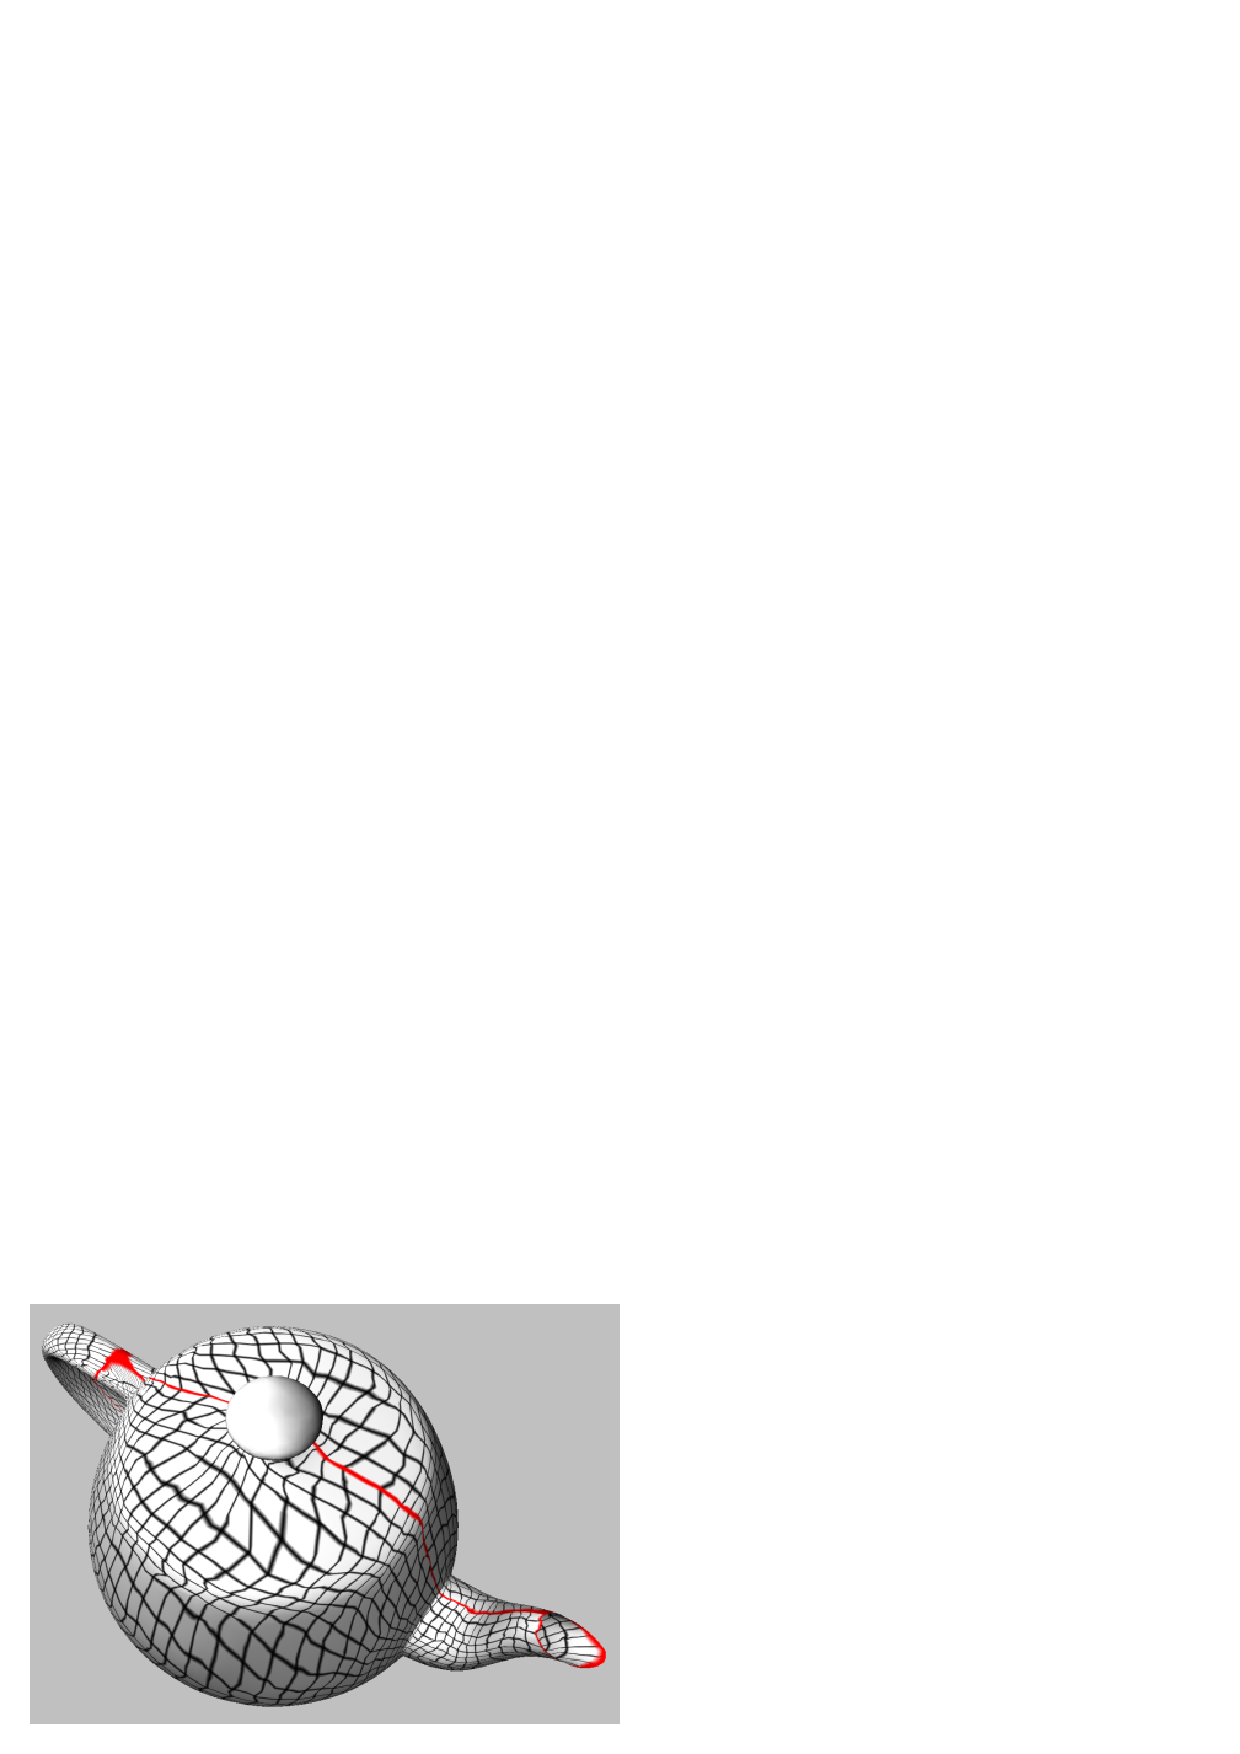
\includegraphics[width=0.5\textwidth]{Surface_mesh_parameterization/uniform} % omit .eps suffix
    \end{ccTexOnly}
    \begin{ccHtmlOnly}
        <img width="50%" border=0 src="./uniform.png"><P>
    \end{ccHtmlOnly}
    % Title
    \begin{figure}[h]
        \caption{Tutte Barycentric Mapping (the red line emphasizes the cutting path)}
    \end{figure}
\end{center}


\subsubsection{Discrete Conformal Map}

\ccc{CGAL::Discrete_conformal_map_parameterizer_3<ParameterizationMesh_3, BorderParameterizer_3, SparseLinearAlgebraTraits_d>}  \\

Discrete Conformal Map parameterization has been introduced by Eck et
al. to the graphics community~\cite{cgal:eddhls-maam-95}. It attempts to
lower angle deformation by minimizing a discrete version of the
Dirichlet energy as derived by Pinkall and
Polthier~\cite{cgal:fh-survey-05}.

% pierre: fix references

A one-to-one mapping is guaranteed only when two conditions are
fulfilled: the barycentric mapping condition (each vertex in parameter
space is a convex combination if its neighbouring vertices) and the
border is convex.

% pierre: add cot figure, and detail what it means to have all weights
% positive, otherwise it is confusing.

This method solves two \#vertices x \#vertices sparse linear
systems. The matrix (the same for both systems) is symmetric definite
positive, thus can be efficiently solved using dedicated linear
solvers (x s for the example shown).

% Insert image conformal.png/eps with title "Discrete Conformal Map"
\begin{center}
    \label{Surface_mesh_parameterization-fig-conformal}
    % Image
    \begin{ccTexOnly}
        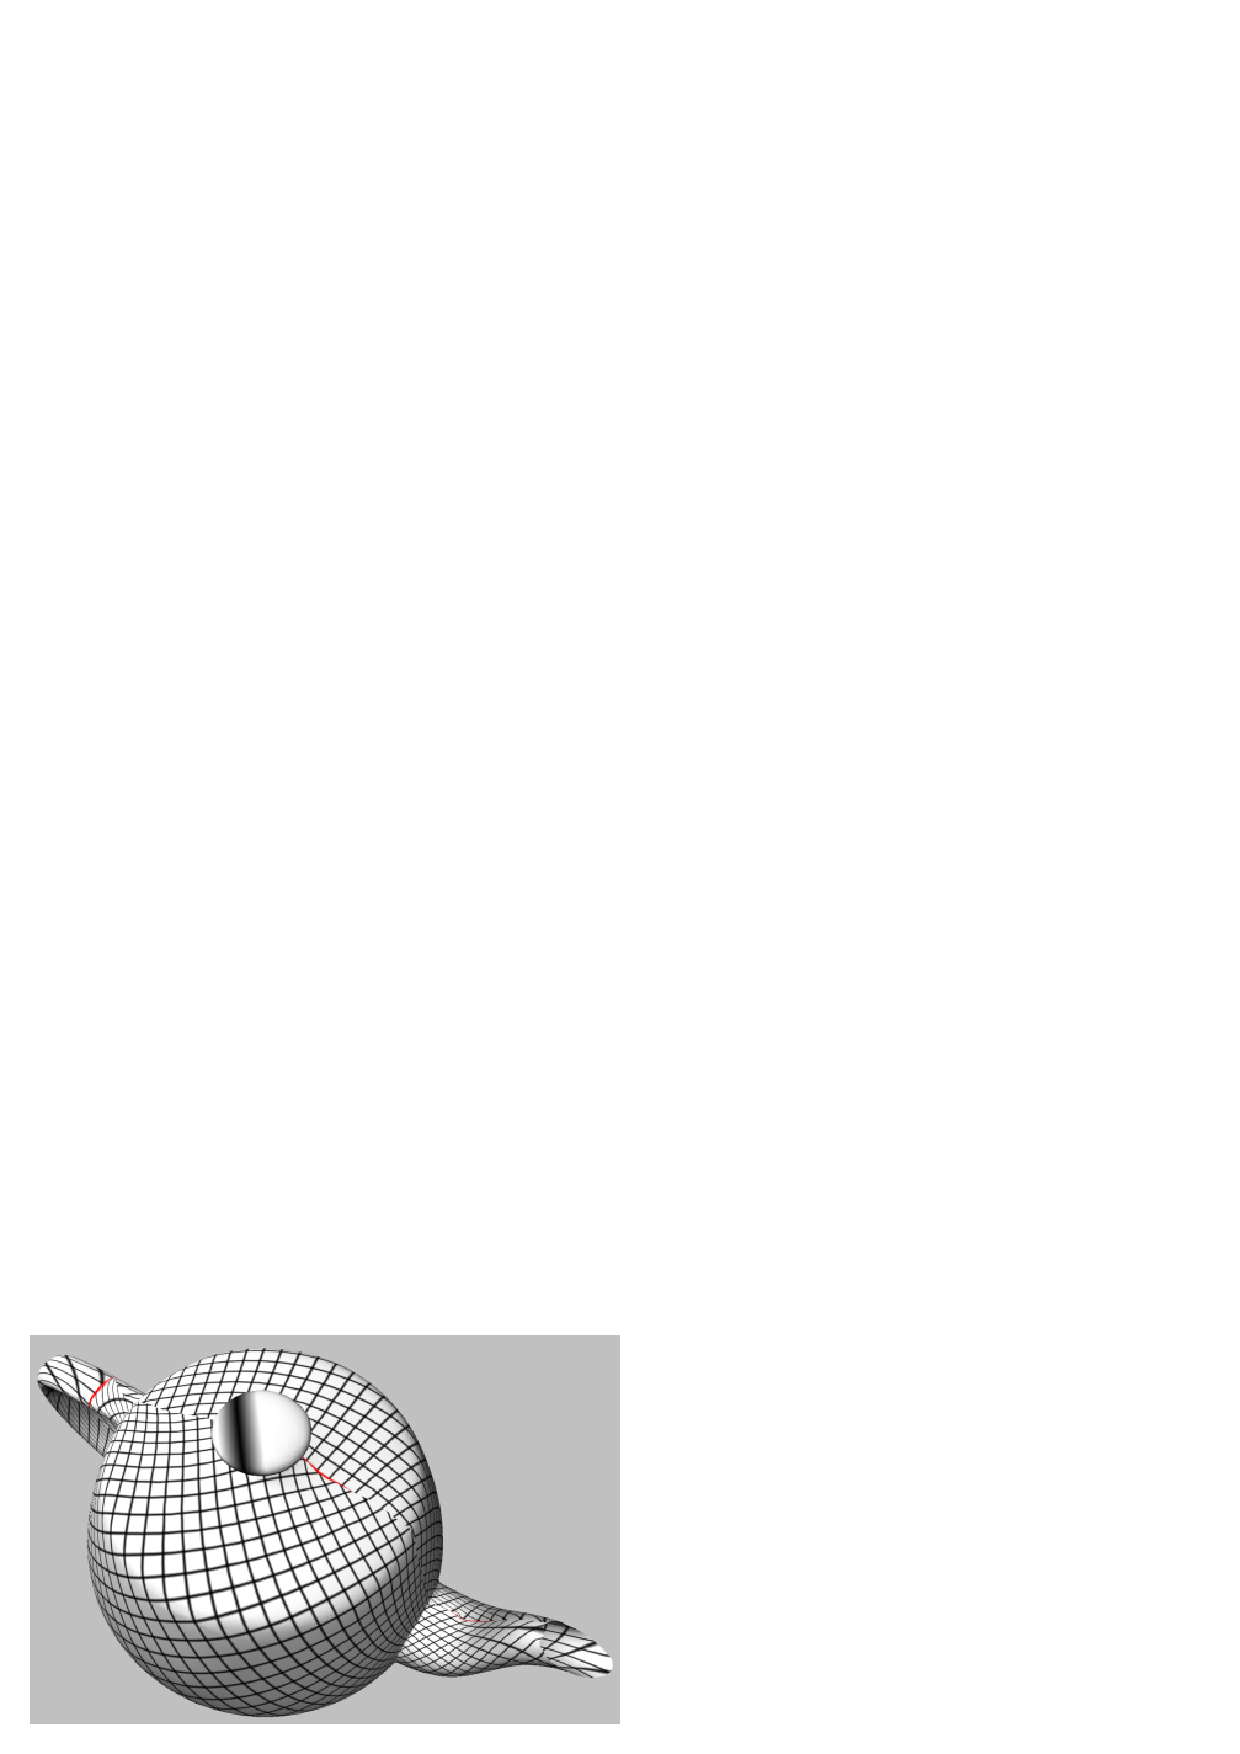
\includegraphics[width=0.5\textwidth]{Surface_mesh_parameterization/conformal} % omit .eps suffix
    \end{ccTexOnly}
    \begin{ccHtmlOnly}
        <img width="50%" border=0 src="./conformal.png"><P>
    \end{ccHtmlOnly}
    % Title
    \begin{figure}[h]
        \caption{Discrete Conformal Map}
    \end{figure}
\end{center}


\subsubsection{Floater Mean Value Coordinates}

\ccc{CGAL::Mean_value_coordinates_parameterizer_3<ParameterizationMesh_3, BorderParameterizer_3, SparseLinearAlgebraTraits_d>}  \\

The Mean Value Coordinates parameterization method has been introduced
by Floater~\cite{cgal:f-mvc-03}. Each vertex in parameter space is
optimized so as to be a convex combination of its neighbouring
vertices. The barycentric coordinates are this time unconditionnaly
positive, by deriving an application of the mean theorem for harmonic
functions. It is in essence an approximation of the Discrete Conformal
Maps, with a one-to-one mapping always guaranteed. This method solves
two \#vertices x \#vertices sparse linear systems. The matrix (the
same for both systems) is asymmetric.

% Insert image floater.png/eps with title "Floater Mean Value Coordinates"
\begin{center}
    \label{Surface_mesh_parameterization-fig-floater}
    % Image
    \begin{ccTexOnly}
        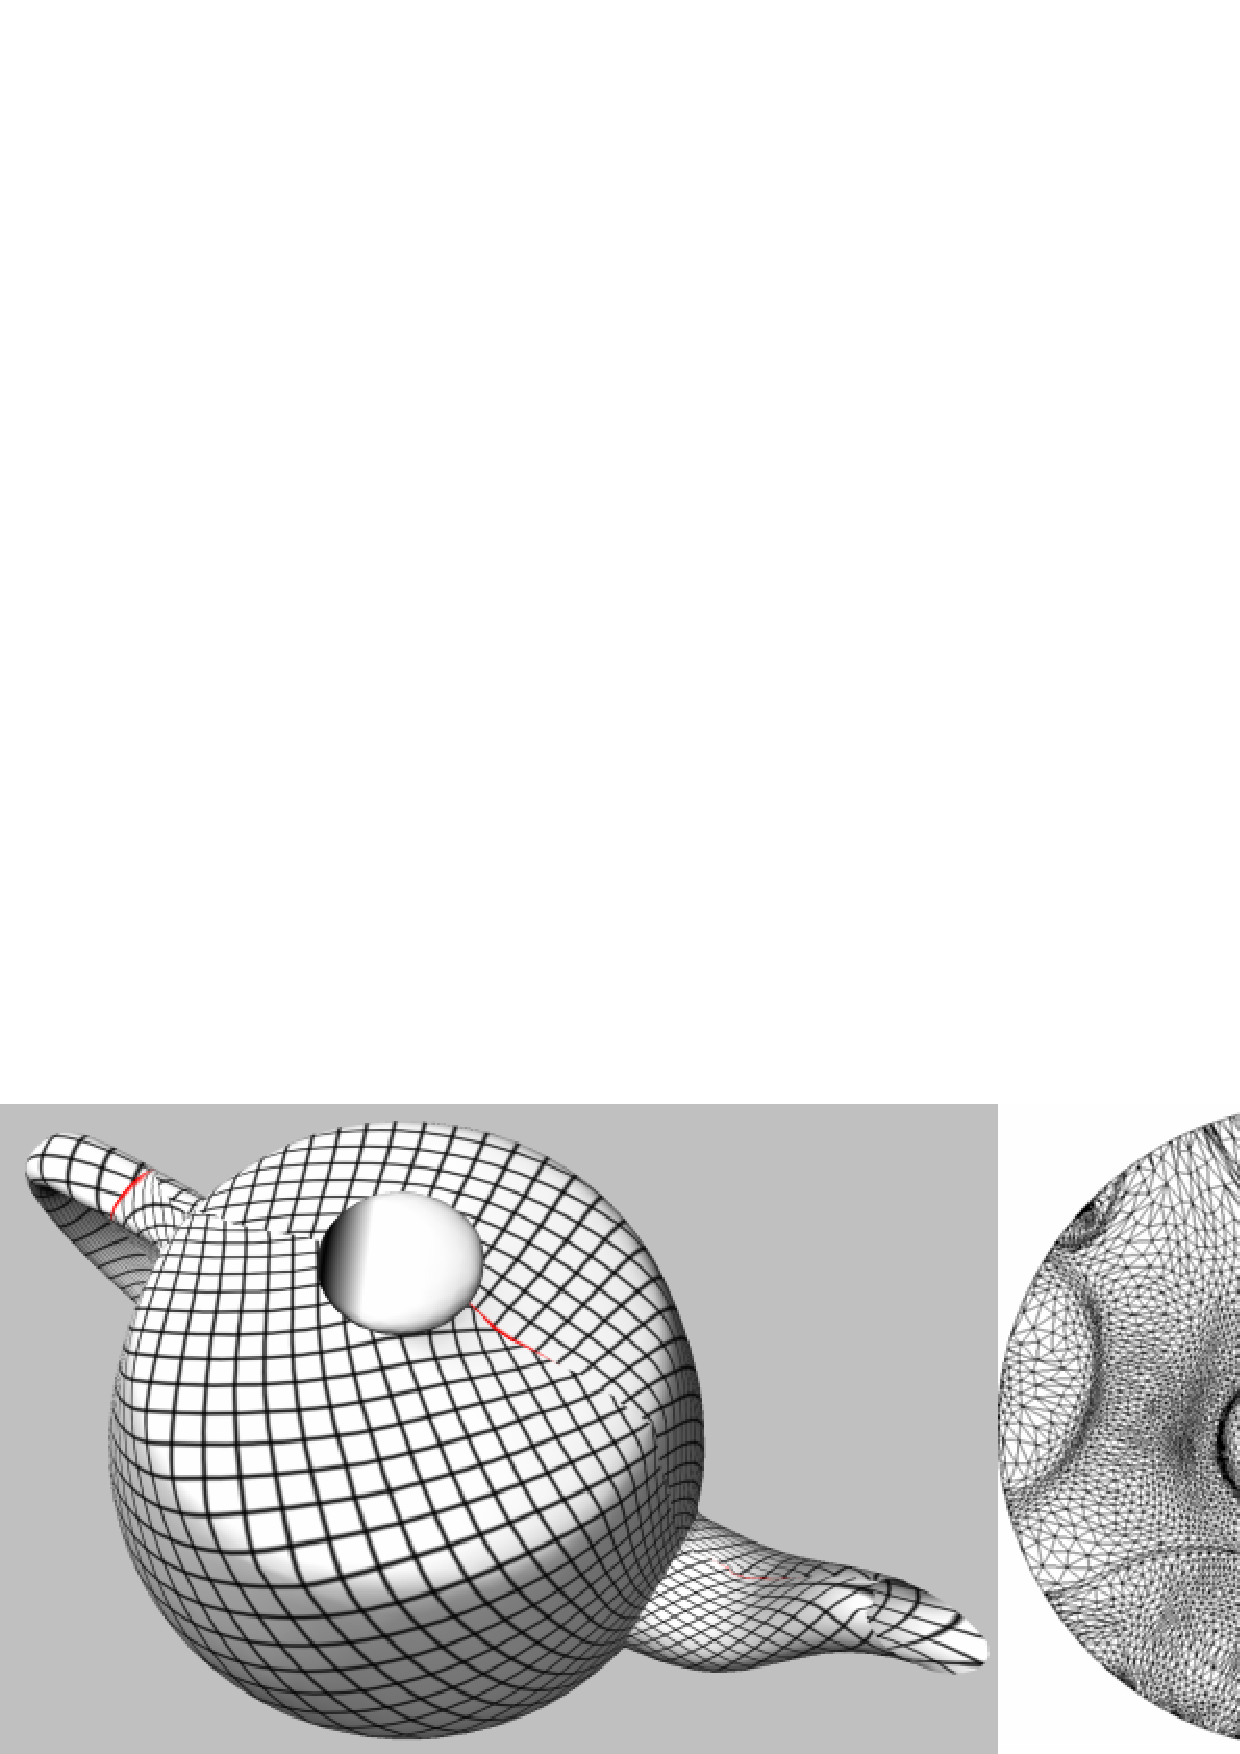
\includegraphics[width=0.5\textwidth]{Surface_mesh_parameterization/floater} % omit .eps suffix
    \end{ccTexOnly}
    \begin{ccHtmlOnly}
        <img width="50%" border=0 src="./floater.png"><P>
    \end{ccHtmlOnly}
    % Title
    \begin{figure}[h]
        \caption{Floater Mean Value Coordinates}
    \end{figure}
\end{center}


\subsubsection{Discrete Authalic parameterization}

\ccc{CGAL::Discrete_authalic_parameterizer_3<ParameterizationMesh_3, BorderParameterizer_3, SparseLinearAlgebraTraits_d>}  \\

The Discrete Authalic parameterization method has been introduced by
Desbrun, Meyer and Alliez~\cite{cgal:dma-ipsm-02}.  It corresponds to
a weak formulation of an area-preserving method, and in essence
locally minimizes the area distortion. A one-to-one mapping is
guaranteed only if the convex combination condition is fulfilled and
the border is convex.  This method solves two
\#vertices x \#vertices sparse linear systems. The matrix (the same
for both systems) is asymmetric.

% Insert image authalic.png/eps with title "Discrete Authalic Parameterization"
\begin{center}
    \label{Surface_mesh_parameterization-fig-authalic}
    % Image
    \begin{ccTexOnly}
        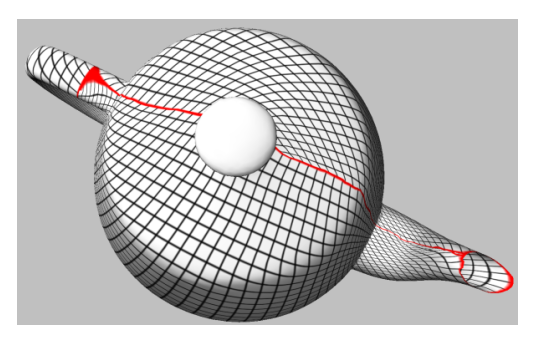
\includegraphics[width=0.5\textwidth]{Surface_mesh_parameterization/authalic} % omit .eps suffix
    \end{ccTexOnly}
    \begin{ccHtmlOnly}
        <img width="50%" border=0 src="./authalic.png"><P>
    \end{ccHtmlOnly}
    % Title
    \begin{figure}[h]
        \caption{Discrete Authalic Parameterization}
    \end{figure}
\end{center}


\subsubsection{Border Parameterizations for Fixed Methods}
\label{sec:Border-Parameterizations-for-Fixed-Methods}

Border Parameterizations for Fixed Border Surface Parameterizations
are a family of methods to define a set of constraints, namely two
$u,v$ coordinates for each vertex along the border.

\begin{itemize}

\item The user can select a border parameterization among
two commonly used methods: uniform or arc-length parameterization, the
arc-length parameterization being used by default.

\item One convex shape specified by:

    \begin{itemize}

    \item one shape among two standard ones: a circle or a square.
    The circular border parameterization is used by default as it
    corresponds to the simplest convex shape. The square border
    parameterization is commonly used for texture mapping.

    \end{itemize}

\end{itemize}

\ccc{CGAL::Circular_border_arc_length_parameterizer_3<ParameterizationMesh_3>}  \\
\ccc{CGAL::Circular_border_uniform_parameterizer_3<ParameterizationMesh_3>}  \\
\ccc{CGAL::Square_border_arc_length_parameterizer_3<ParameterizationMesh_3>}  \\
\ccc{CGAL::Square_border_uniform_parameterizer_3<ParameterizationMesh_3>}  \\


\subsection{Free Border Surface Parameterizations}

\subsubsection{Least Squares Conformal Maps}

\ccc{CGAL::LSCM_parameterizer_3<ParameterizationMesh_3, BorderParameterizer_3, SparseLinearAlgebraTraits_d>}  \\

The Least Squares Conformal Maps (LSCM) parameterization method has
been introduced by L\'evy et al.~\cite{cgal:lprm-lscm-02}. It
corresponds to a conformal method with a free border (at least two
vertices have to be constrained to obtain a unique solution), which
allows further lowering of the angle distortion. A one-to-one mapping
is not guaranteed by this method. It solves a (2 $\times$
\#triangles) $\times$ \#vertices sparse linear system in the least squares sense.

% Insert image LSCM.png/eps with title "Least Squares Conformal Maps"
\begin{center}
    \label{Surface_mesh_parameterization-fig-LSCM}
    % Image
    \begin{ccTexOnly}
        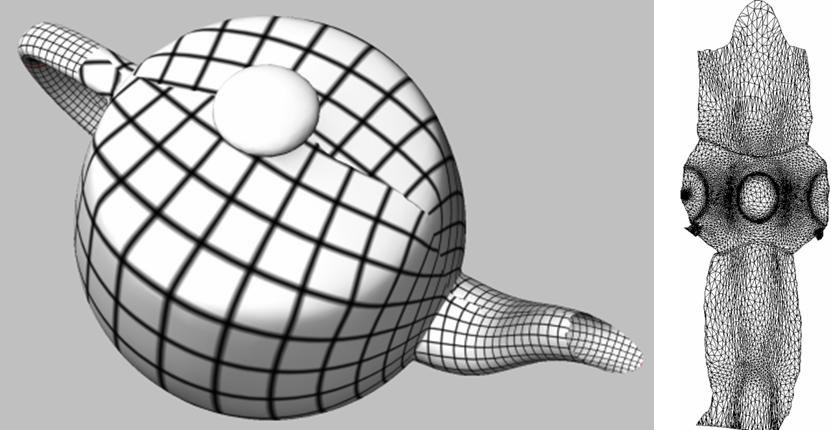
\includegraphics[width=0.5\textwidth]{Surface_mesh_parameterization/LSCM} % omit .eps suffix
    \end{ccTexOnly}
    \begin{ccHtmlOnly}
        <img width="50%" border=0 src="./LSCM.png"><P>
    \end{ccHtmlOnly}
    % Title
    \begin{figure}[h]
        \caption{Least Squares Conformal Maps}
    \end{figure}
\end{center}


\subsubsection{Border Parameterizations for Free Methods}

\ccc{CGAL::Two_vertices_parameterizer_3<ParameterizationMesh_3>}  \\

The associated Border Parameterization method defines only two constraints
(the pinned vertices). They have to be on the specified border.


\subsection{Discrete Authalic Parameterization Example}

The following C++ code computes a Discrete Authalic parameterization
to a \ccc{Polyhedron_3} mesh:

\begin{ccExampleCode}

// CGAL kernel
typedef CGAL::Cartesian<double>                         Kernel;

// Mesh true type and parameterization adaptors
typedef CGAL::Polyhedron_3<Kernel>                      Polyhedron;
typedef CGAL::Parameterization_polyhedron_adaptor_3<Polyhedron>
                                                        Parameterization_polyhedron_adaptor;

// Discrete Authalic Parameterization
typedef CGAL::Discrete_authalic_parameterizer_3<Parameterization_polyhedron_adaptor>
                                                        Parameterizer;

int main(int argc,char * argv[])
{
    Polyhedron mesh;
    ...

    // The Surface_mesh_parameterization package needs an adaptor to handle Polyhedron_3 meshes
    // The mesh must be a topological disk
    Parameterization_polyhedron_adaptor mesh_adaptor(&mesh);

    // Discrete Authalic Parameterization
    Parameterizer::Error_code err = CGAL::parameterize(&mesh_adaptor, Parameterizer());
    ...
}

\end{ccExampleCode}

The complete example is available in
\ccc{Authalic_parameterization.C}.


\subsection{Square Border Arc Length Parameterization Example}

The following C++ code computes a Floater Mean Value Coordinates
parameterization with a Square Border Arc Length parameterization:

\begin{ccExampleCode}

// CGAL kernel
typedef CGAL::Cartesian<double>                         Kernel;

// Mesh true type and parameterization adaptors
typedef CGAL::Polyhedron_3<Kernel>                      Polyhedron;
typedef CGAL::Parameterization_polyhedron_adaptor_3<Polyhedron>
                                                        Parameterization_polyhedron_adaptor;

// Square border parameterizer
typedef CGAL::Square_border_arc_length_parameterizer_3<Parameterization_polyhedron_adaptor>
                                                        Border_parameterizer;

// Floater Mean Value Coordinates parameterizer with square border
typedef CGAL::Mean_value_coordinates_parameterizer_3<Parameterization_polyhedron_adaptor,
                                                     Border_parameterizer>
                                                        Parameterizer;

int main(int argc,char * argv[])
{
    Polyhedron mesh;
    ...

    // The Surface_mesh_parameterization package needs an adaptor to handle Polyhedron_3 meshes
    // The mesh must be a topological disk
    Parameterization_polyhedron_adaptor mesh_adaptor(&mesh);

    // Floater Mean Value Coordinates parameterization
    // with a Square Border Arc Length Parameterization
    Parameterizer::Error_code err = CGAL::parameterize(&mesh_adaptor, Parameterizer());
    ...
}

\end{ccExampleCode}

See the complete example \ccc{Square_border_parameterization.C}.
